\documentclass[a4paper,10pt]{article}
\usepackage{multirow}
\usepackage[latin1]{inputenc}
\usepackage{amsmath,amssymb,amsfonts,latexsym}
%\usepackage[pdftex]{graphicx}
\usepackage{graphicx}
\DeclareGraphicsExtensions{.png,.pdf,.jpg}
\usepackage{float}
\textwidth 6.0in

\begin{document}

\title{Lab Course\\Scientific Computing\\ Worksheet 2}
\author{Alfredo Parra\\ Shulin Gao}
\date{Due November 21st, 2011}
\maketitle
\oddsidemargin 0.0in

We examine the differential equation
\begin{equation}
\dot{p}=7\left(1-\frac{p}{10}\right)\cdot p,
\label{eq:eqdif}
\end{equation}
with initial condition $p(0)=20$, which has an analytical solution given by
\begin{equation}
p(t)=\frac{200}{20-10e^{-7t}}.
\label{eq:solEx}
\end{equation}
We observe that the solution presents a rapid decrease from $p=20$ to $p=10$, a feature which makes the use of explicit methods rather troublesome, as we shall see.
\textbf{a)} Here is the plot of the function $p(t)$:

\begin{figure}[H]%
\centering
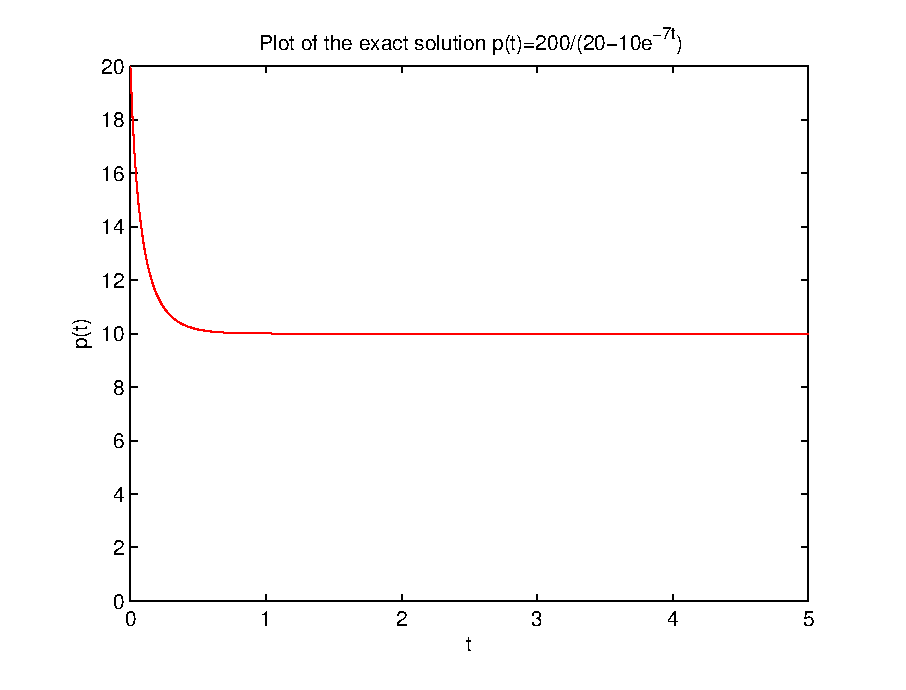
\includegraphics[width=.7\columnwidth]{ExactGraph.eps}%
\caption{The exact solution of the differential equation \eqref{eq:eqdif} decreases rapidly and tends to the value $p=10$.}%
\label{ExactFig}%
\end{figure}
\textbf{b)} We know use the explicit Euler method and Heun's method to calculate approximate solutions of \eqref{eq:eqdif} with $t_{end}=5$ and $\delta t=1,\frac{1}{2},...,\frac{1}{8}$ (MATLAB files \texttt{expEuler.m, Heun.m}). Since all solutions except $\delta t = \frac{1}{8}$ exhibit a divergent growth (Fig. \ref{EuHeFig1}), the case $\delta t = \frac{1}{8}$ is plotted separately (Fig. \ref{EuHeFig2})

\begin{figure}[H]%
\centering
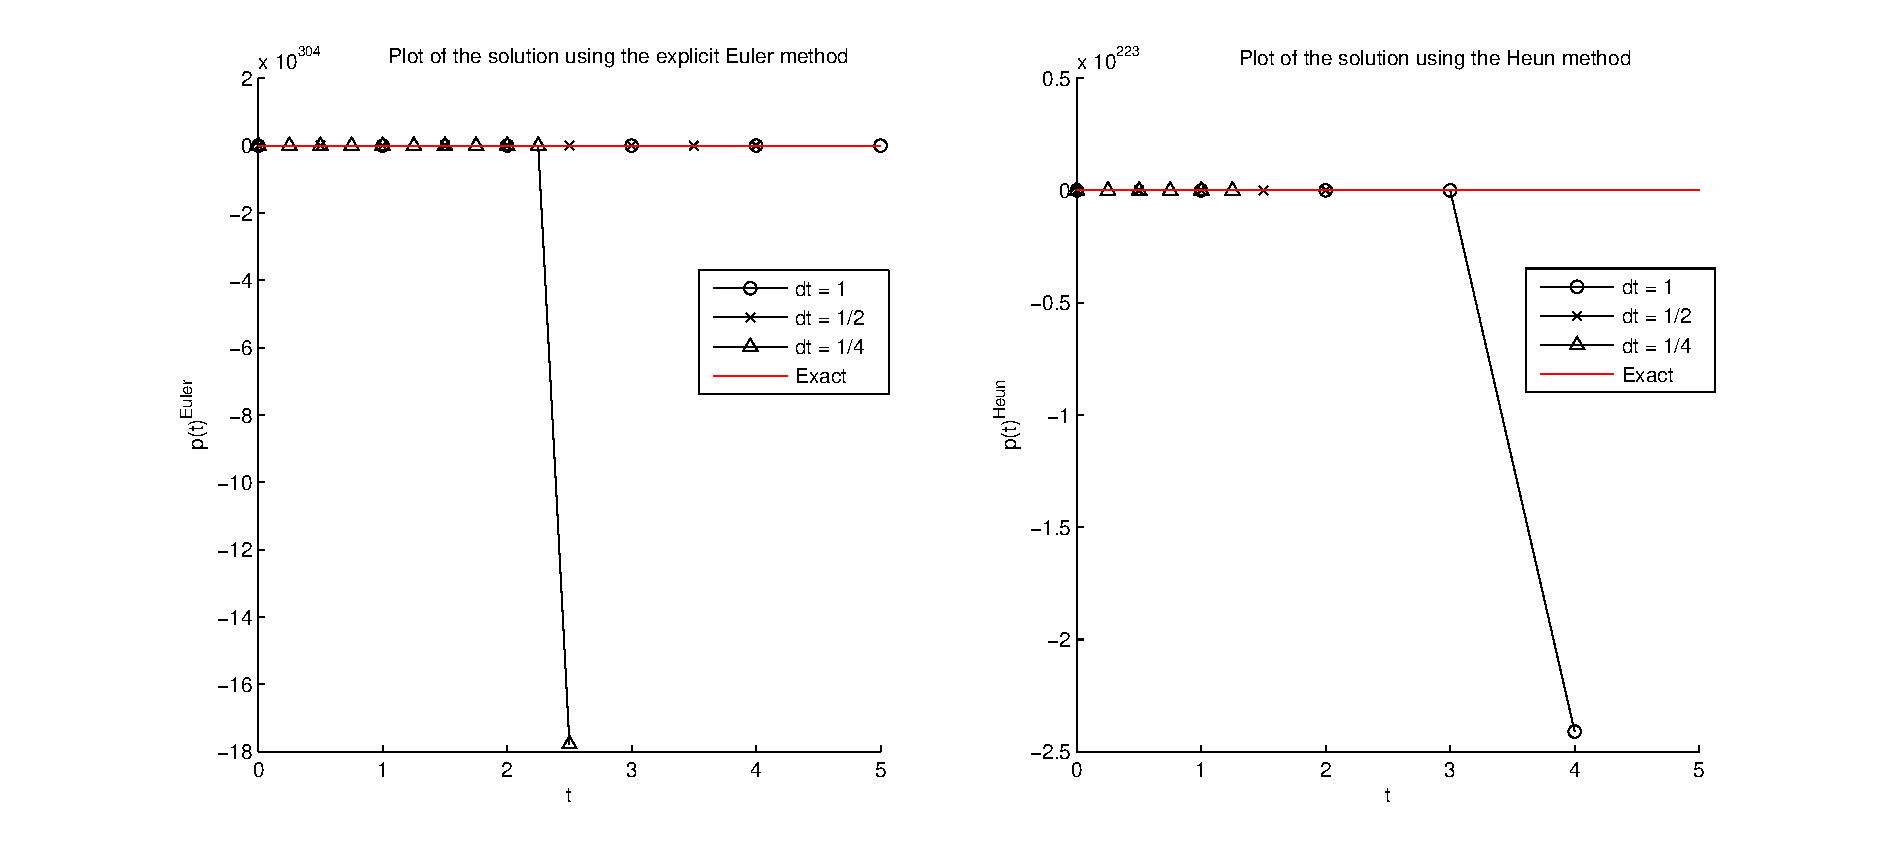
\includegraphics[width=1\columnwidth]{EuHeGraph.eps}%
\caption{The explicit Euler and Heun solutions of \eqref{eq:eqdif} are divergent for $\delta t = 1,\frac{1}{2},\frac{1}{4}$.}%
\label{EuHeFig1}%
\end{figure}

\begin{figure}[H]%
\centering
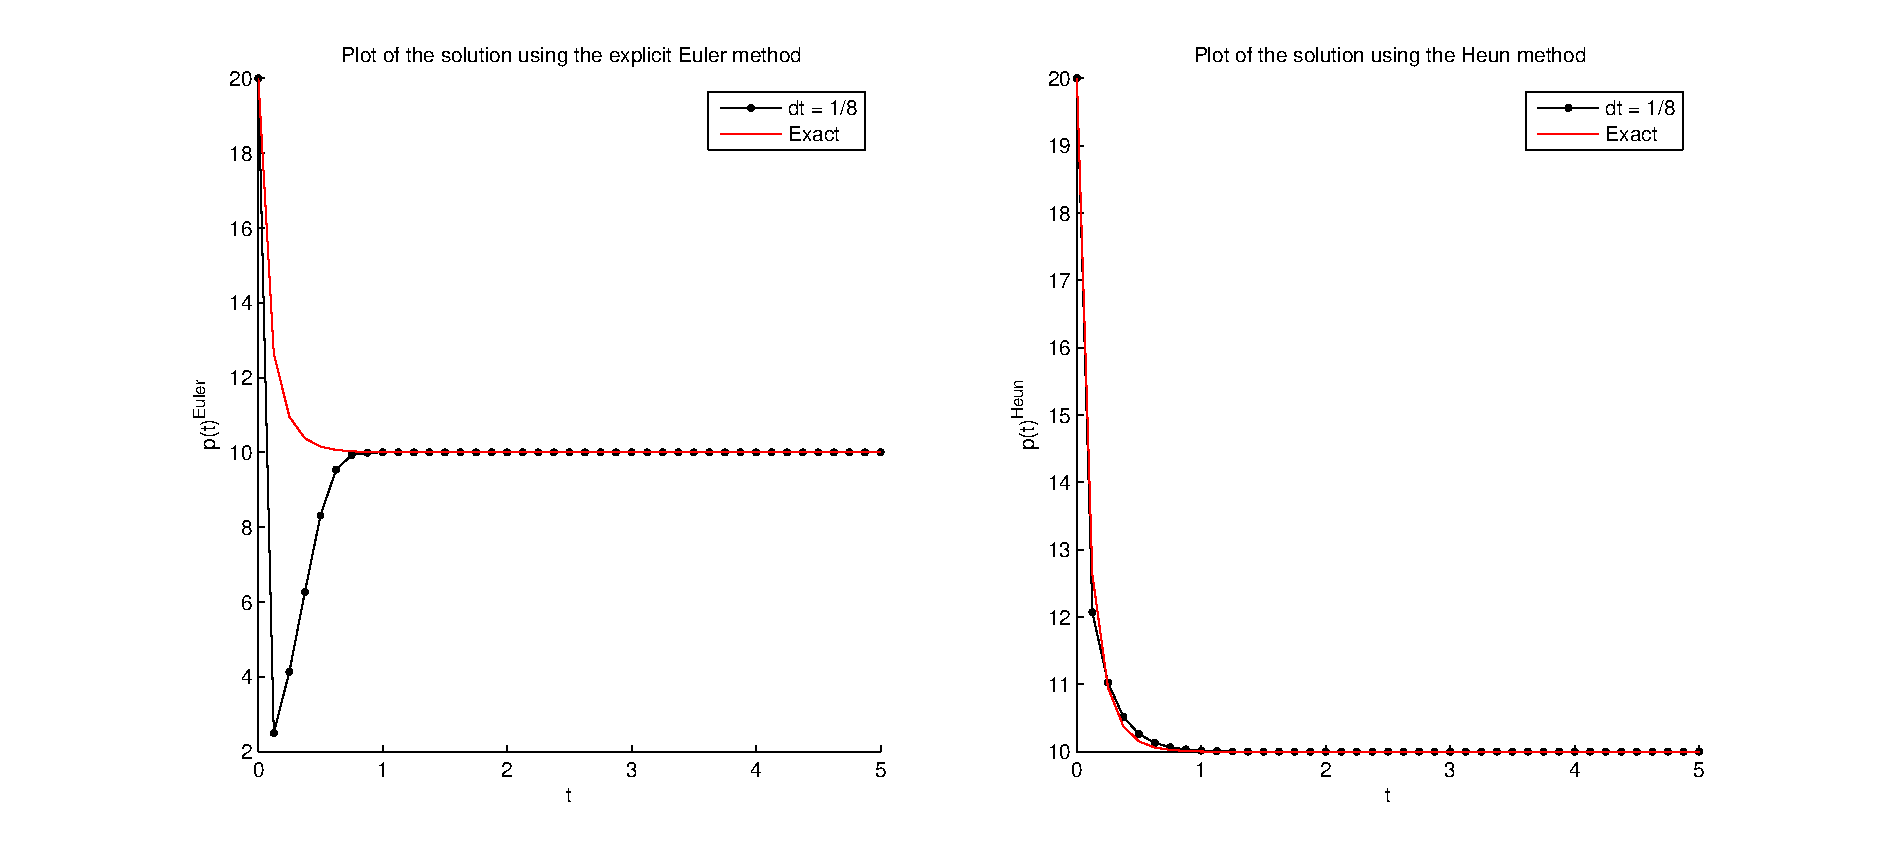
\includegraphics[width=1\columnwidth]{EuHeGraph2.eps}%
\caption{The explicit Euler and Heun solutions of \eqref{eq:eqdif} seem to converge for $\delta t = \frac{1}{8}$.}%
\label{EuHeFig2}%
\end{figure}

\textbf{c) } The implicit Euler and the second order Adams-Moulton methods were implemented in the files \texttt{impEuler.m, AdMo.m}. Since both methods are implicit, each approximation $p_{n+1}$ of the solution has to be calculated using Newton's method. Nevertheless, it is easy to observe that, for this particular equation, both the implicit Euler method and the second order Adams-Moulton method give rise to a quadratic equation for $p_{n+1}$ which can be easily solved. For the implicit Euler method, we have
\begin{subequations}
\begin{equation} p_{n+1} = p_n + \delta t f(t_{n+1},y_{n+1}),\end{equation}
\begin{equation}p_{n+1}^2+\frac{10(1-7\delta t)}{7\delta t}p_{n+1}-p_n=0,\end{equation}
\label{eq:EuQuad}
\end{subequations}
which has the exact solutions
\begin{equation}
p_{n+1} = -\frac{5(1-7\delta t)}{7\delta t}\pm\frac{1}{2}\sqrt{\frac{100(1-7\delta t)^2}{49\delta t^2}+\frac{40p_n}{7\delta t}}.
\label{eq:solnsEu}
\end{equation}
Likewise, for Adams-Moulton's method, we have
\begin{subequations}
\begin{equation} p_{n+1} = p_n + \frac{\delta t}{2}[f(t_{n+1},y_{n+1})+f(t_n,y_n)],\label{eq:ameq1}\end{equation}
\begin{equation}p_{n+1}^2+\frac{20(1-7\delta t/2)}{7\delta t}p_{n+1}-\frac{20[1+(7\delta t/2)(1-p_n/10)]}{7\delta t}p_n=0,\label{eq:ameq2}\end{equation}
\label{eq:AMQuad}
\end{subequations}
with exact solutions
\begin{equation}
p_{n+1} = -\frac{10}{7\delta t}\left(1-\frac{7\delta t}{2}\right)\pm\sqrt{\frac{5}{7\delta t}}\cdot\sqrt{\frac{20}{7\delta t}\left(1-\frac{7\delta t}{2}\right)^2+4\left[1+7\delta t\left(1-\frac{p_n}{10}\right)\right]p_n}.
\label{eq:solnsAM}
\end{equation}

One interesting result can be observed from equation \eqref{eq:solnsAM}. Taking $p_0 = p(0) = 20$, the value of $p_1$ will only be real if the discriminant of \eqref{eq:ameq2} is positive, and this imposes a condition on $\delta t$. It is not difficult to show that if $\delta t$ is greater that the critical value $\delta t_c \approx 0.285714 $, the root in \eqref{eq:solnsAM} becomes imaginary, and $p_1$ becomes complex, which does not correspond to the solution of the  problem studied. We can also see from \eqref{eq:solnsEu} that this is never the case for the implicit Euler method (the root is always real).

These results will only serve to compare the answers obtained with Newton's method. Both methods are implemented in each of the files \texttt{impEuler.m, AdMo.m}. For Newton's method, we set an accuracy of $10^{-4}$ and check if the algorithm converges to a given value. Two different criteria were tried for this worksheet. One is to set an upper limit on the number of Newton iterations. The second is to compare the error $e^{k+1}=|y^{k+1}-y^k|$ with $e^k = |y^k-y^{k-1}|$ to see if the error is growing (i.e. $|e^{k+1}/e^k|>1$). If it is the case, for this particular equation, this criterion is sufficient, as we shall see.

\vspace{3mm}

\textbf{d) } The solutions were computed using the implicit Euler method and the second order Adams-Moulton method with the use of Newton's method. The case $\delta t = \frac{1}{2}$ for the Adams-Moulton method did not converge, and so the plot is not shown.

\begin{figure}[H]%
\centering
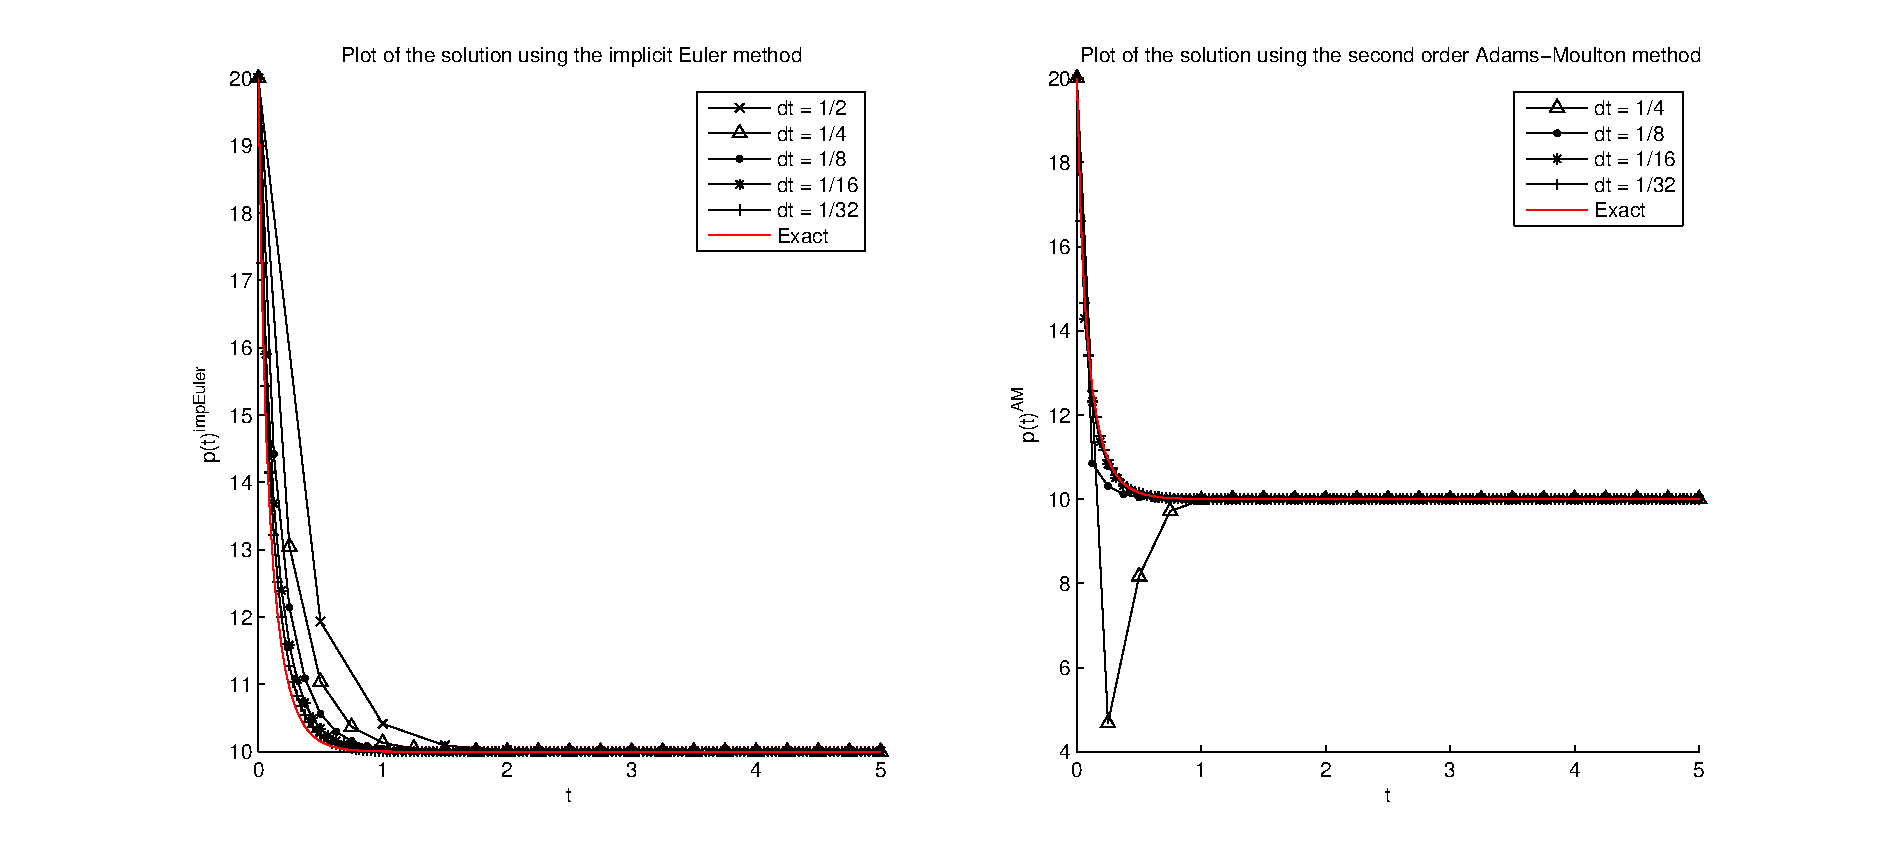
\includegraphics[width=1\columnwidth]{impEAMGraph.eps}%
\caption{The implicit Euler method converged for all $\delta t$, whereas for $\delta t = \frac{1}{2}$, the Adams-Moulton method did not.}%
\label{impEAM}%
\end{figure}

The fact that the Adams-Moulton method does not converge for $\delta t=1/2$ is consistent with our previous discussion concerning the solutions of the quadratic equation. In fact, Newton's method does not converge for values of $\delta t$ larger than the same $\delta t_c$ mentioned above.

\vspace{3mm}

\textbf{e) } Two linearized versions of the Adams-Moulton method were implemented, namely
\begin{subequations}
\begin{align}
y^{(n+1)} &= y^{(n)} + \frac{\delta t}{2}\left[7\cdot\left(1-\frac{y^{(n)}}{10}\right)\cdot y^{(n)}+7\cdot\left(1-\frac{y^{(n+1)}}{10}\right)\cdot y^{(n)}\right],\\
y^{(n+1)} &= y^{(n)} + \frac{\delta t}{2}\left[7\cdot\left(1-\frac{y^{(n)}}{10}\right)\cdot y^{(n)}+7\cdot\left(1-\frac{y^{(n)}}{10}\right)\cdot y^{(n+1)}\right].
\end{align}
\label{eq:lins}
\end{subequations}

Once again, even though Newton's method can solve the equation, $y^{(n+1)}$ can be easily found as a function of $y^{(n)}$, since we have a linear equation. Both methods were implemented in the file \texttt{adMoLin.m}. Here, we no longer have the issue of the quadratic case (imaginary roots in the implicit Adams-Moulton method).

\vspace{3mm}

\textbf{f) } The plots of the solutions to \eqref{eq:eqdif} using the linearizations \eqref{eq:lins} are shown in Fig. \ref{AMLFig}. We observe that, for every timestep, the first linearization gives very good results, whereas the second linearization presents an oscillatory solution for $\delta t = 1/2$.

\begin{figure}[H]%
\centering
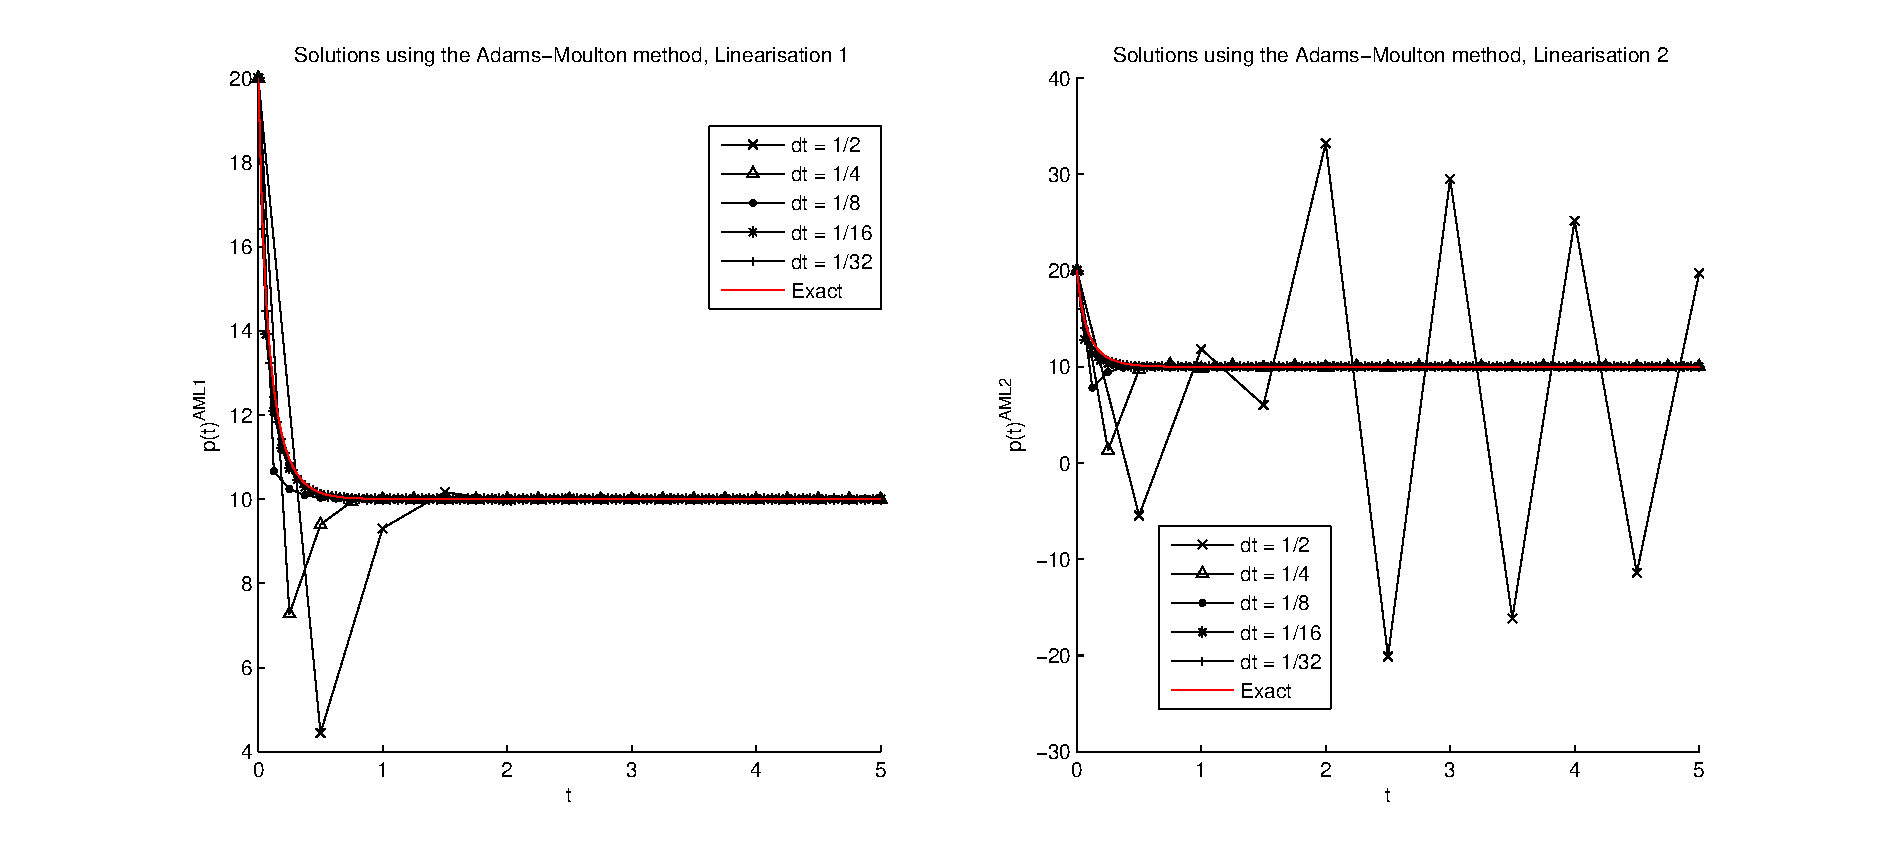
\includegraphics[width=1\columnwidth]{AMLGraph.eps}%
\caption{Plots of the two linearized versions of the Adams-Moulton method \eqref{eq:lins}.}%
\label{AMLFig}%
\end{figure}

\vspace{3mm}

\textbf{g, h)} The approximation error
\begin{equation}
E = \sqrt{\frac{\delta t}{5}\sum_{k}(p_k-p_{k,exact})^2},
\label{eq:Error}
\end{equation}
was calculated for each of the methods, and the different values are given in the tabulars below. The factor by which the error is reduced when the timestep is halved is also shown in the tabulars. For the four implicit methods, we observed that the errors using Newton's method and solving the quadratic and linear equations were similar to at least seven significant figures.

\vspace{3mm}

\textbf{i) } Following the heuristic definition of stability, we concluded that both explicit methods are not stable for $\delta t > 1/4$ (at least). The second linearization of the Adams-Moulton method presents oscillations that do not resemble the solutions, which is why we consider it unstable. The cases for which each of the methods are stable are reported in the tabular at the end (marked with a cross).

\begin{center}

\addtolength{\tabcolsep}{10pt}
\renewcommand{\arraystretch}{2}

\begin{tabular}[0.75\textwidth]{ | c | c | c | c | c | c | c |}
		\hline
		\multicolumn{7}{|c|}{Explicit Euler's method (q=1)} \\
		\hline
		$\delta t$ & 1 & 1/2 & 1/4 & 1/8 & 1/16 & 1/32\\
		\hline
		error & 8e30 & Inf & Inf & 2.059 & 0.4854 & 0.1754\\
		\hline
		error red. & Inf & NaN & 0 & 0.2357 & 0.3614 & 0.4436\\
		\hline
\end{tabular}

\vspace{5mm}

\begin{tabular}{ | c | c | c | c | c | c | c |}
		\hline
		\multicolumn{7}{|c|}{Method of Heun (q=2)} \\
		\hline
		$\delta t$ & 1 & 1/2 & 1/4 & 1/8 & 1/16 & 1/32\\
		\hline
		error & Inf & Inf & Inf & 0.9496e-1 & 0.9376e-1 & 0.2350e-1\\
		\hline
		error red. & NaN & NaN & 0 & 0.9873 & 0.2506 & 0.2262\\
		\hline
\end{tabular}

\vspace{5mm}

\begin{tabular}{ | c | c | c | c | c | c |}
		\hline
		\multicolumn{6}{|c|}{Implicit Euler method (q=1)} \\
		\hline
		$\delta t$ & 1/2 & 1/4 & 1/8 & 1/16 & 1/32\\
		\hline
		error & 0.5781 & 0.5151 & 0.3665 & 0.2233 & 0.1245\\
		\hline
		error red. & 0.8912 & 0.7115 & 0.6093 & 0.5574 & 0.5315\\
		\hline
\end{tabular}

\vspace{5mm}

\begin{tabular}{ | c | c | c | c | c | c |}
		\hline
		\multicolumn{6}{|c|}{Second order Adams-Moulton method (q=2)} \\
		\hline
		$\delta t$ & 1/2 & 1/4 & 1/8 & 1/16 & 1/32\\
		\hline
		error & - & 0.1473e1 & 0.3035 & 0.7037e-1 & 0.1668e-1\\
		\hline
		error red.& 0.2060 & 0.2319 & 0.2371 & 0.2446 & 0.2484\\
		\hline
\end{tabular}

\vspace{5mm}

\begin{tabular}{ | c | c | c | c | c | c |}
		\hline
		\multicolumn{6}{|c|}{Second order Adams-Moulton method, Linearisation 1 (q=1)} \\
		\hline
		$\delta t$ & 1/2 & 1/4 & 1/8 & 1/16 & 1/32\\
		\hline
		error & 0.1820e1 & 0.8402 & 0.3342 & 0.1237 & 0.4879e-1\\
		\hline
		error red.& 0.4617 & 0.3977 & 0.3701 & 0.3945 & 0.4381\\
		\hline
\end{tabular}

\vspace{5mm}

\begin{tabular}{ | c | c | c | c | c | c |}
		\hline
		\multicolumn{6}{|c|}{Second order Adams-Moulton method, Linearisation 2 (q=1)} \\
		\hline
		$\delta t$ & 1/2 & 1/4 & 1/8 & 1/16 & 1/32\\
		\hline
		error & 0.1886e2 & 0.2154e1 & 0.7990 & 0.2926 & 0.1220\\
		\hline
		error red.& 0.1142 & 0.3709 & 0.3662 & 0.4169 & 0.4615\\
		\hline
\end{tabular}

\vspace{5mm}

\begin{tabular}{ | c | c | c | c | c | c | c |}
		\hline
		& Exp. Euler & Heun & Imp. Euler & A-M & A-M L1 & A-M L2\\
		\hline
		$\delta t = 1/2$&&&$\times$&&$\times$&\\
		\hline
		$\delta t = 1/4$&&&$\times$&$\times$&$\times$&$\times$\\
		\hline
		$\delta t = 1/8$&$\times$&$\times$&$\times$&$\times$&$\times$&$\times$\\
		\hline
		$\delta t = 1/16$&$\times$&$\times$&$\times$&$\times$&$\times$&$\times$\\
		\hline
		$\delta t = 1/32$&$\times$&$\times$&$\times$&$\times$&$\times$&$\times$\\
		\hline
\end{tabular}

\end{center}

\vspace{10mm}

\textbf{Questions}

\vspace{5mm}

1) From our observations of the errors $E$, we conclude that $q=1$ for the explicit and implicit Euler methods, as well as both linearizations of the Adams-Moulton method, since the error is halved when the $\delta t$ is halved (for $\delta t$ sufficiently small); likewise, $q=2$ for the methods of Heun and Adams-Moulton, since the error is reduced by 4 when $\delta t$ is halved (also for $\delta t$ sufficiently small).

\vspace{3mm}

2) We can observe that, indeed, the implicit methods are much more stable than the explicit methods, but some cases seem to disagree with the notion of unconditional stability. This is particularly the case for the Adams-Moulton method when $\delta t$ is larger than approximately 0.285714. From our analysis in question \textit{c}, it is evident that this happens because the roots of the resulting nonlinear (quadratic) equation become negative. For those same values of $\delta t$, we observe that Newton's method does not converge. The problem is that we are dealing with nonlinear equations, and their solutions depend explicitly on $\delta t$, so we cannot expect to obtain solutions for every timestep a priori. This will depend on the particular $f(y,t)$ in question. Nevertheless, the implicit Euler method does not present any restrictions, which can be seen from Eq. \eqref{eq:solnsEu}.

\vspace{3mm}

3) One way to compare both linearizations is to observe the terms by which they differ, namely
\begin{subequations}
\begin{align}
L1(y^{(n+1)}) &= \left(1-\frac{y^{(n+1)}}{10}\right)\cdot y^{(n)},\\
L2(y^{(n+1)}) &= \left(1-\frac{y^{(n)}}{10}\right)\cdot y^{(n+1)}.
\end{align}
\label{eq:Lterms}
\end{subequations}
Now, suppose we want to calculate $y^{(1)}$ starting from $y^{(0)}=y(0)$. We know that this approximation $y^{(1)}$ will deviate from the exact solution $y(t = \delta t)$ by some error $\epsilon^{(1)}$, that is, $y^{(1)}=y(\delta t) + \epsilon^{(1)}$. Inserting this into the above terms gives
\begin{subequations}
\begin{align}
L1(y^{(1)}) &= \left(1-\frac{y(\delta t)+\epsilon^{(1)}}{10}\right)\cdot y(0) = y(0)-\frac{y(0)\cdot y(\delta t)}{10}-\frac{\epsilon^{(1)}\cdot y(0)}{10},\\
L2(y^{(1)}) &= \left(1-\frac{y(0)}{10}\right)\cdot (y(\delta t)+\epsilon^{(1)}) = y(\delta t)-\frac{y(0)\cdot y(\delta t)}{10}-\frac{\epsilon^{(1)}\cdot y(0)}{10}+\epsilon^{(1)}.
\end{align}
\label{eq:Lterms2}
\end{subequations}
We observe that the second linearization is off by an extra factor $\epsilon^{(1)}$ compared to the first linearization, which is why the first linearization works better.

\vspace{3mm}

4) The only difference between the two equations studied in the worksheets is only a factor of 7, but the solutions behave very differently, as we have seen. In this worksheet, we are dealing with a \textit{stiff equation}, whereby the particular solution exhibits a very rapid variation in a short interval, and then tends to a constant value. In these cases, it is better to treat the problem with implicit methods, and the reason is the following (as explained in \cite{Gol_Ort}).

A similar, less complicated (linear) problem than ours would be to find the solution of the equation $y' = -100y + 100$ with $y_0 = 2$. The solution is given by $y(x) = e^{-100x}+1$, and the explicit Euler method would give the following solution (after solving the recurrence relation)
\begin{equation}
y_n = (1-100h)^n+1,
\label{eq:EulAp}
\end{equation}
where $h$ is the step. Indeed, $(1-100h)^n$ is an approximation of $e^{-100x}$, but if $h>0.02$, $|1-100h|>1$ and the numerical solution explodes, even if that term barely contributes to the solution. Thus, the step $h$ has to be very small in order to compensate for the small term and obtain a stable algorithm. Choosing an implicit method may take care of this problem. Indeed, the implicit Euler method in this case gives
\begin{equation}
y_n = \frac{1}{(1+100h)^n}+1,
\label{eq:sol2}
\end{equation}
and the behavior is always stable, even for large $h$. The bottom line is that explicit methods give rise to polynomial expressions which cannot properly approximate some solutions, and implicit methods can give, for instance, rational expressions, which are far more suitable for these problems.
Our exact solution has the form
\begin{equation}
p(t)=\frac{200}{20-10e^{-7t}} = \frac{40}{4-e^{-14t}}+\frac{20e^{-7t}}{4-e^{-14t}},
\label{eq:solEx2}
\end{equation}
and so the second term vanishes very rapidly, whereas the second tends to the value of 10, exactly as in the previous problem, which is why we should choose implicit methods. Nevertheless, if the equation is not stiff (such as in the first worksheet), we may opt for explicit schemes, since they are less expensive in computational terms. With respect to the linearizations, we can see that, since the schemes are linear in $y^{(n+1)}$, the convergence of Newton's method is immediate (our functions are straight lines), which is why these linearizations are good alternatives.

\begin{thebibliography}{99}
\bibitem{Gol_Ort}
	Golub G., Ortega J., Scientific Computing and Differential equations. San Diego: Academic Press; 1992.
\end{thebibliography}
\end{document}